\subsection{Attraktivitet}


\centerline{\textbf{Hur viktigt är attraktivitet för 
din användarupplevelse}}

\begin{figure}[H]
  \centering
  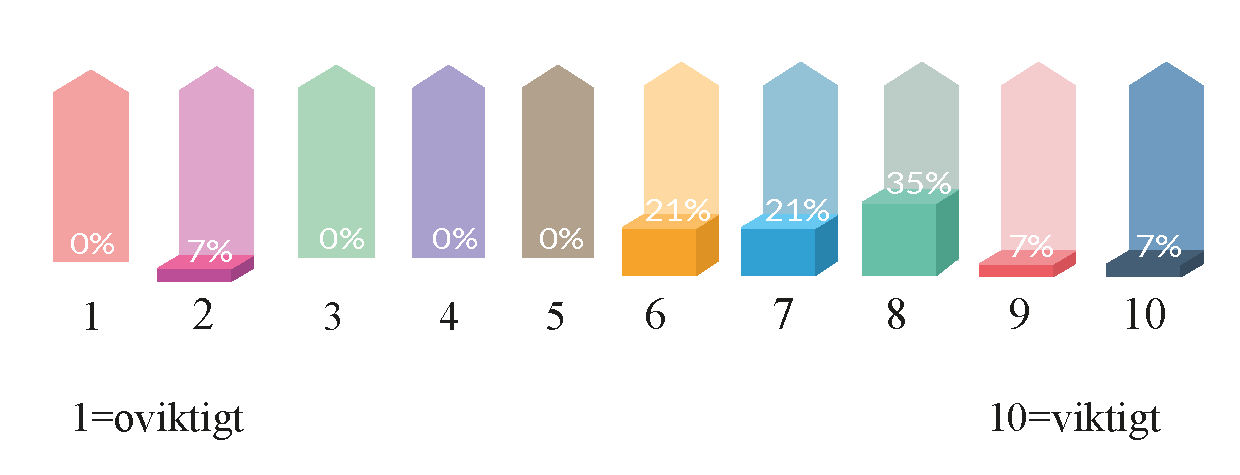
\includegraphics[scale=0.7]{Rityta_11.pdf}
 \captionsetup{justification=centering,margin=2cm}
\caption{Resultat i procentuell skala på respondenternas svar}
\end{figure} 

Medelvärdet av ovan figur är 7.14. Siffran representerar ett medelsnitt av stapeldiagrammet som visar hur viktigt det var för användarupplevelsen enligt kategoriseringen framtagen av Laugwitz et al. \cite{Laugwitz2008ConstructionQuestionnaire}. 

%\[
 % m = \frac{2 + 18 + 21 + 40 + 9 + 10}{14} = 7.14
%  \]
  
%Med en standardavvikelse på

%\[
%\sigma = \sqrt{V}= \sqrt{\frac{(2-1)^{2} + (6-3)^{2} + (7-3)^{2} + (8-5)^{2} + (9-1)^{2} + (10-1)^{2}} {6}} = \sqrt{30} = 5.5
 %   \]

\newpage
\begin{figure}[H]
  \centering
  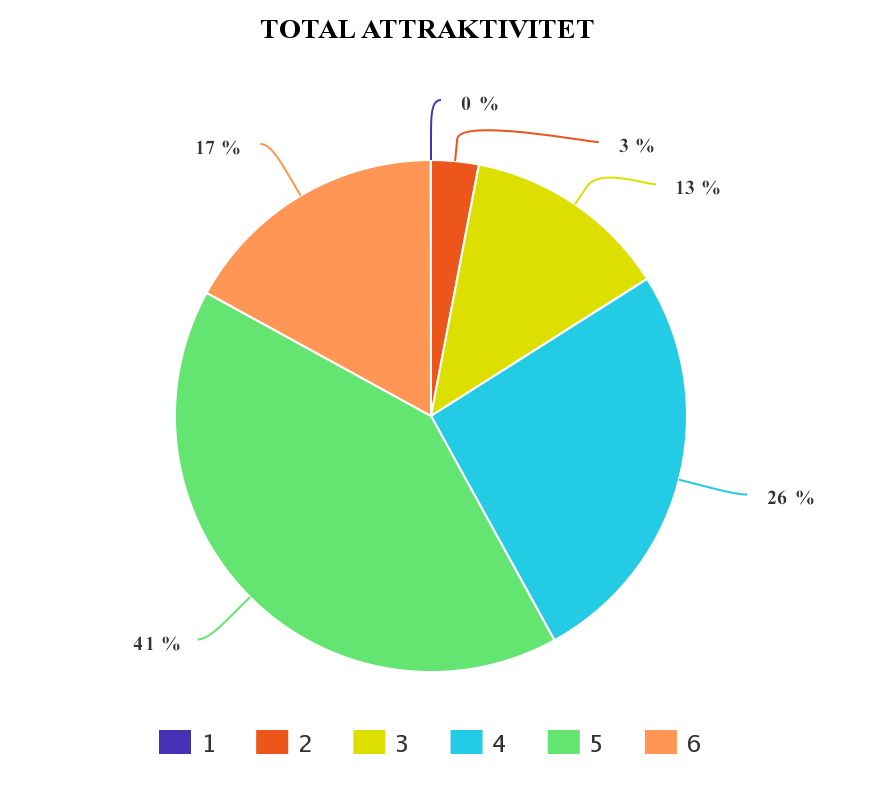
\includegraphics[scale=0.4]{meta-chart-6.png}
 \captionsetup{justification=centering,margin=2cm}
  \caption{Resultat av total attraktivitet}
\end{figure}

Figuren visar det slutgiltiga resultatet från både enkätundersökningen samt fokusgrupperna. Figuren visar sambandet mellan hur viktigt attraktivitet är för användarupplevelsen i en applikation kontra hur pålitlig prototypen känts. Den första rutan visar på hur viktigt det är för användaren att en applikation är attraktiv, enligt personerna som medverkade i fokusgrupperna. Denna siffran beräknades med hjälp av snitt och varians och presenteras nedan. Diagrammen visar på hur attraktiv prototypen kändes, enligt användarna som svarade på enkätundersökningen. 
\newline

\textbf{Citat från fokusgrupperna}
\begin{quotation}
\em  Det var tydligt och rent, det var lätt att komma igång med det. Lättillgängligt. 
\end{quotation}

\begin{quotation}
\em  Jag tycker att den är inbjudande för att den är enkel och det är inte jättemycket textmassor utan det är ganska instinktivt hur jag ska börja klicka
\end{quotation}

\begin{quotation}
\em  I think it looked really nice, but I think its a bit hard to understand whats the mission is. And I think that if you could show it in a graphical way before she start to tak, other wise its hard to get the point.  But I think it’s nice to have someone talking for once, because usually it’s a lot of text and so.
\end{quotation}

%\begin{quotation}
%\em %Vill alltid ha kontroll på hur långt jag kommit, så det är bra. Vill veta vart är jag, hur mycket har jag kvar, är det lönt att börja på en ny osv.
%\end{quotation}

%\begin{quotation}
%\em  %Det var lagom långa filmer, så fort dom blir för långa så tappar jag uppmärksamheten.
%\end{quotation}

%\begin{quotation}
%\em  %Ja nu vet jag ungefär vad jag har att förvänta mig och därför har jag hög acceptansnivån för utseendet 
%\end{quotation}

%\begin{quotation}
%\em   %Man kanske kan paketera det lite grann så att det inte blir så internt coach perspektiv.
%\end{quotation}

%\begin{quotation}
%\em %Kanske att man distribuerar det eller att du får möteskallelser automatiskt in i telefonen för att faktiskt göra dessa actions som du kommit överens
%\end{quotation}

%\begin{quotation}
%\em  %Ja det var verkligen lagom långt klipp
%\end{quotation}

%\begin{quotation}
%\em %Då är det bra att det finns en tidslinje, så man ser hur långt den är
%\end{quotation}

%\begin{quotation}
%\em %För just videon signalerar ju någon form utav personlig dialog. Men om det bara är en allmän instruktion som är lika oavsett vad jag svara i olika steg så är den kanske lite besviken på den. 
%\end{quotation}

%\begin{quotation}
%\em  %Inte så mycket ”buzz”. Det är funktion snarare än att det är feeling. Det är inte så säljande, inte så wowigt, inte så mycket konfetti, utan det är funktion.
%\end{quotation}

%\begin{quotation}
%\em %I liked that it had clear intentions, very specific for the person who uses it. And a clear flow of the prototype. But I would like an option to skip the videos and have a text or something. 
%\end{quotation}
